\documentclass[a4paper]{article}
\usepackage[a4paper,outer=1cm,inner=1cm,top=1cm,bottom=1cm]{geometry}
\twocolumn
\usepackage{graphicx}
\usepackage{karnaugh-map}
\usepackage{tabularx}
\usepackage{hyperref}
\begin{document}
\title{Assignment-2}
\author{Name:A.Gowri Priya\and Email :  \url{gowripriyaappayyagari@gmail.com}}
\date{}
\maketitle
\begin{abstract}
Reduce the following Boolean Expression to its simplest form using K-Map by using assembly language:
E(U,V,Z,W)=   (2 , 3 , 6 , 8 , 9 , 10 , 11 , 12 , 13 )
\end{abstract}
\section{Components}

%\begin{table}[]
    \centering
    \begin{tabular}{ |c |c |c |c |}
\hline
\hline
\newline
\newline
\textbf{Components} & \textbf{Value} & \textbf{Quantity} \\
\hline
 %Resistor & 220Ohm & 1 \\ 
 Arduino & UNO & 1 \\  
 %Seven segment Display &  & 1 \\
 %Decoder& 7447&1 \\
 seven segment display& - & 1 \\
 Jumper wires&M-M &18\\
 Breadboard& &1\\
 Resister&150 ohm&1\\
 Decoder&7447&1\\
 \hline
 \end{tabular}
 %\vspace{3mm}
 
 %\caption{Table 1.0}
    \label{table1}
%\end{table}

\section{K-Map}
    \paragraph{}
 From the given data the minterms are 2,3,6,8,9,10,11,12,13.
     
\begin{karnaugh-map}[4][4][1][][]
    \maxterms{0,1,4,5,7,14,15}
    \minterms{2,3,6,8,9,10,11,12,13}

    % note: posistion for start of \draw is (0, Y) where Y is
    % the Y size(number of cells high) in this case Y=2
    \draw[color=black, ultra thin] (0, 4) --
    node [pos=0.7, above right, anchor=south west] {$XW$} % Y label
    node [pos=0.7, below left, anchor=north east] {$ZY$} % X label
    ++(135:1);
        
\end{karnaugh-map}

The minimized expression is
    E=(UZ'+V'Z+U'ZW')

   
    \begin{karnaugh-map}[4][4][1][][]
         \maxterms{0,1,4,5,7,14,15}
         \minterms{2,3,6,8,9,10,11,12,13}
        \implicantedge{3}{2}{11}{10}
        \implicantedge{8}{9}{12}{13}
        \implicant{2}{6}
    \draw[color=black, ultra thin] (0, 4) --
    node [pos=0.7, above right, anchor=south west] {$XW$} % Y label
    node [pos=0.7, below left, anchor=north east] {$ZY$} % X label
    ++(135:1);
\end{karnaugh-map}
\section{HardwareConnections}
*Make the connections as shown in the Figure3 and Figure4.

*Connect COM pin of seven segment display to Vcc through Resister and Dot pin to ground.
\begin{figure}
    \centering
    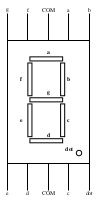
\includegraphics{seven.png}
    \caption{Seven segment display}
    \label{fig:my_label}
\end{figure}
\begin{figure}
    \centering
    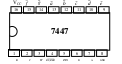
\includegraphics{7447ic.png}
    \caption{Pin diagram of 7447IC}
    \label{fig:my_label}
\end{figure}
\begin{figure}
    \centering
    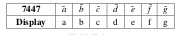
\includegraphics{sevenseg.png}
    \caption{}
    \label{fig:my_label}
\end{figure}
\begin{figure}
    \center
    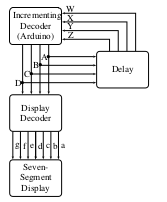
\includegraphics[scale=1]{connect.jpg} 
  
    \caption{}
    \label{fig:my_label}
\end{figure}
\begin{tabularx}{0.5\textwidth} {
  | >{\centering\arraybackslash}X
  | >{\centering\arraybackslash}X
  | >{\centering\arraybackslash}X
  | >{\centering\arraybackslash}X
  | >{\centering\arraybackslash}X | }
\hline
 U& V & Z & W & E \\
\hline
0 & 0 & 0 & 0 & 0\\ 
\hline
0 & 0 & 0 & 1& 0 \\
\hline
0 & 0 & 1 & 0 & 1\\
\hline
0 & 0 & 1 & 1 & 1 \\
\hline
0 & 1 & 0 & 0 & 0 \\ 
\hline
0 & 1 & 0 & 1 & 0 \\
\hline
0 & 1 & 1 & 0 & 1 \\
\hline
0 & 1 & 1& 1 & 0 \\
\hline
1 & 0 & 0 & 0 & 1\\ 
\hline
1 & 0 & 0 & 1& 1\\
\hline
1 & 0 & 1 & 0 & 1\\
\hline
1 & 0 & 1 & 1 & 1 \\
\hline
1 & 1 & 0 & 0 & 1 \\ 
\hline
1 & 1 & 0 & 1 & 1 \\
\hline
1 & 1 & 1 & 0 & 0 \\
\hline
1 & 1 & 1& 1 & 0 \\
\hline
\end{tabularx}
Truth Table

\section{Execution}
*Verify the above truth table by using the minimized expression in the following code.
\framebox{
\url{https://github.com/gowripriya-2002/FWC/blob/main/Asg_2/asg_2.asm}}
\bibliographystyle{ieeetr}
\end{document}
